\section{Data Structures} \label{datastructure}

This section discusses some of the data structures which can be created using C. We will cover single linked lists, double linked lists and tree structures. These dynamic structures are used to create database structures, lists, stacks, queues, state machines and buffers.

\subsection{typedef}

\textit{typedef} allows new datatypes to be constructed. It is a useful construct as related data can be grouped together. This is best illustrated with examples.

\begin{lstlisting}[language=C,showstringspaces=false,caption={File: typedef1.c, new datatype example},captionpos=b,label=typedef]

 1 #include <stdio.h>
 2 #include <stdint.h>
 3 
 4 typedef struct
 5 {
 6 uint8_t x;
 7 uint8_t y;
 8 uint16_t color;
 9 } pixel_str;
10 
11 void display(pixel_str *ptr)
12 {
13 printf ("x coordinate : %d\n",ptr->x);
14 printf ("y coordinate : %d\n",ptr->y);
15 printf ("color        : 0x%6.6x\n",ptr->color);
16 } 
17 
18 int main (void)
19 {
20 pixel_str point;
21 
22 point.x = 23;
23 point.y = 12;
24 point.color = 0x00ff00; // RGB GREEN
25 
26 display(&point); // display pixel
27 return 0;
28 }

INTERACTIONS

$ cc typedef1.c
$ ./a.out
x coordinate : 23
y coordinate : 12
color        : 0x00ff00
$
\end{lstlisting}

Listing \ref{typedef} shows a new datatype called \textit{pixel\_str} defined on lines:4-9. It comprises three fields, namely \textit{uint8\_t x}, \textit{uint8\_t y} and \textit{uint16\_t color}. A variable called \textit{point} is declared on line:20. This variable is then initialized on lines:22-24 and then passed by reference to the function \textit{display(...)}. 

For declared variables the fields are accessed using \textit{variable.field} on lines:22-24, whereas for variable pointers the fields are accessed by \textit{variable-\textgreater field} on lines:13-15.

\begin{lstlisting}[language=C,showstringspaces=false,caption={File: typedef2.c, initializer},captionpos=b,label=typedef2]

 1 #include <stdio.h>
 2 #include <stdint.h>
 3 
 4 typedef struct 
 5 {
 6 char     *machine;
 7 uint32_t memsize_GB;
 8 uint32_t start_addr;
 9 } machine_str;
10 
11 machine_str current =
12 {
13 .machine = "zeus",
14 .memsize_GB = 4,
15 .start_addr = 0x8000
16 };
17 
18 int main(void)
19 {
20 printf ("... machine\t: \'%s\'\n",current.machine);
21 printf ("... memsize_GB\t: %dGB\n",current.memsize_GB);
22 printf ("... address\t: 0x%8.8x\n",current.start_addr);
23 
24 return 0;
25 }

INTERACTIONS

$ cc typedef2.c
$ ./a.out
... machine	: 'zeus'
... memsize_GB	: 4GB
... address	: 0x00008000
$

\end{lstlisting}

Listing \ref{typedef2} shows a quick method to initialize a new data structure. This can be useful when providing an initial value to a large number of fields. The listing shows a datatype called \textit{machine\_str}. The datatype contains three fields, as shown on lines:4-9. A variable \textit{current} is of this type and is initialized on lines:11-16 with the values \textit{"zeus"}, \textit{4} and \textit{0x8000} respectively. 

\subsection{Tables}

Tables are useful structures. We define a table as being an array of a new datatype. This is useful as the new datatype consists of different fields, so a table is effectively an array of multiple different types. This is best illustrated with an example.

\begin{lstlisting}[language=C,showstringspaces=false,caption={File: table.c, state machine},captionpos=b,label=table]

 1 #include <stdio.h>
 2 #include <stdint.h>
 3 
 4 /* macros */
 5 #define NO_TRANSITION -1
 6 
 7 /* new datatypes */
 8 typedef struct
 9 {
10 char c;
11 uint8_t state;
12 uint8_t new_state;
13 int (*function)(int);
14 } states_str;
15 
16 /* function prototypes */
17 int ident(int loc);
18 int record(int loc);
19 
20 /* globals */
21 
22 int at=-1;
23 
24 states_str states[] =
25 {
26 'h',    0,      1,      record,
27 'h',    1,      1,      record,
28 'e',    1,      2,      NULL,
29 'l',    2,      3,      NULL,
30 'l',    3,      4,      NULL,
31 'o',    4,      0,      ident,
32  0 ,    0,      0,      NULL
33 };
34 
35 /* functions */
36 int record(int loc)
37 {
38 at=loc;
39 return 0;
40 }
41 
42 int ident(int loc)
43 {
44 printf("... search string 'hello' found at  %d\n",at);
45 return 1;
46 }
47 
48 int state_machine(char *title,char *text)
49 {
50 int indx=0; // start index 
51 int scan;
52 int current=0; // start state
53 int transition;
54 int num;
55 
56 printf("%s: \"%s\"\n",title,text);
57 num = 0;
58 
59   while (text[indx])
60   {
61   scan=0; // reset scan
62   transition = NO_TRANSITION; 
63 
64     while (states[scan].c!=0)
65     {
66       if (text[indx]==states[scan].c && current==states[scan].state)
67         transition = scan;
68     scan++;
69     }
70 
71     if (transition==NO_TRANSITION)
72       current = 0; // reset state
73     else
74     {
75     current = states[transition].new_state;
76       if (states[transition].function!=NULL)
77         num +=states[transition].function(indx);  
78     }
79   indx++;
80   }
81 
82 printf("... strings: %d\n",num);
83 return num;
84 } 
85 
86 int main (void)
87 {
88 state_machine("test 1","kjdhskjfhjkfhhellokjdsfkdj");
89 state_machine("test 2","");
90 state_machine("test 3","dljhjklsdjkfdehjkhed");
91 state_machine("test 4","jhdjshjdsjkhellodkskljfdlhfdhello");
92 state_machine("test 5","jkhdjshjkhelljhjkkjhkjdhkhello");
93 state_machine("test 6","jksahdhhellohellohellokkdjklj");
94 return 0;
95 }

INTERACTIONS

$ cc table.c
$ ./a.out
test 1: "kjdhskjfhjkfhhellokjdsfkdj"
... search string 'hello' found at 13
... strings: 1
test 2: ""
... strings: 0
test 3: "dljhjklsdjkfdehjkhed"
... strings: 0
test 4: "jhdjshjdsjkhellodkskljfdlhfdhello"
... search string 'hello' found at 11
... search string 'hello' found at 28
... strings: 2
test 5: "jkhdjshjkhelljhjkkjhkjdhkhello"
... search string 'hello' found at 25
... strings: 1
test 6: "jksahdhhellohellohellokkdjklj"
... search string 'hello' found at 7
... search string 'hello' found at 12
... search string 'hello' found at 17
... strings: 3
$
\end{lstlisting} \label{tablee}

Listing \ref{table} is a table implementation of the code in listing \ref{switch2}. The first solution was based on the \textit{switch construct}, but this implementation is based on a table state machine. This code is slightly more complex than the previous solution but has the capability of being easily expanded. Any expansion is achieved by adding or removing entries in the table.

The table is of type \textit{states\_str}. The \textit{state\_str} datatype defined on lines:8-14 is made up of four fields, namely \textit{char c}, \textit{uint8\_t state}, \textit{uint8\_t new\_state} and the function pointer \textit{int (*function)(int)}. 

\begin{description}
 \item[$\bullet$] Field \textit{c}, is the character being searched.
 \item[$\bullet$] Field \textit{state}, is the current state of the state machine.
 \item[$\bullet$] Field \textit{new\_state}, is the state of the transition.
 \item[$\bullet$] Field \textit{function}, is the function which is invoked during a state transition.
\end{description}

If both the character \textit{c} and the current \textit{state} are satisfied then a transition can occur to a \textit{new\_state}. There is one last piece of complexity, the \textit{function} field is a function pointer. If the function field is not NULL then it is invoked, as shown on line:76:77.

The table itself is on lines:24-33. There are two special cases to point out with the table. The first is that there are two 'h' entries. This is important as there is a scenario when there are leading 'h's before the final 'h' for \textit{hello}, this is shown on line:26:27. The second point is that the 'l' entries are used to count exactly 2 'l' for the "ll" part of \textit{hello}, as shown in line:29:30.

\subsection{Linked lists}

Linked lists are based on pointers and dynamic memory. Both pointers and dynamic memory are used to construct more complex structures. For deeply embedded systems, dynamic memory is discouraged when the device is fully running but it is not discouraged during the initialization phase. Linked lists can also be implemented without dynamic memory.

\begin{figure}[H]
\centerline{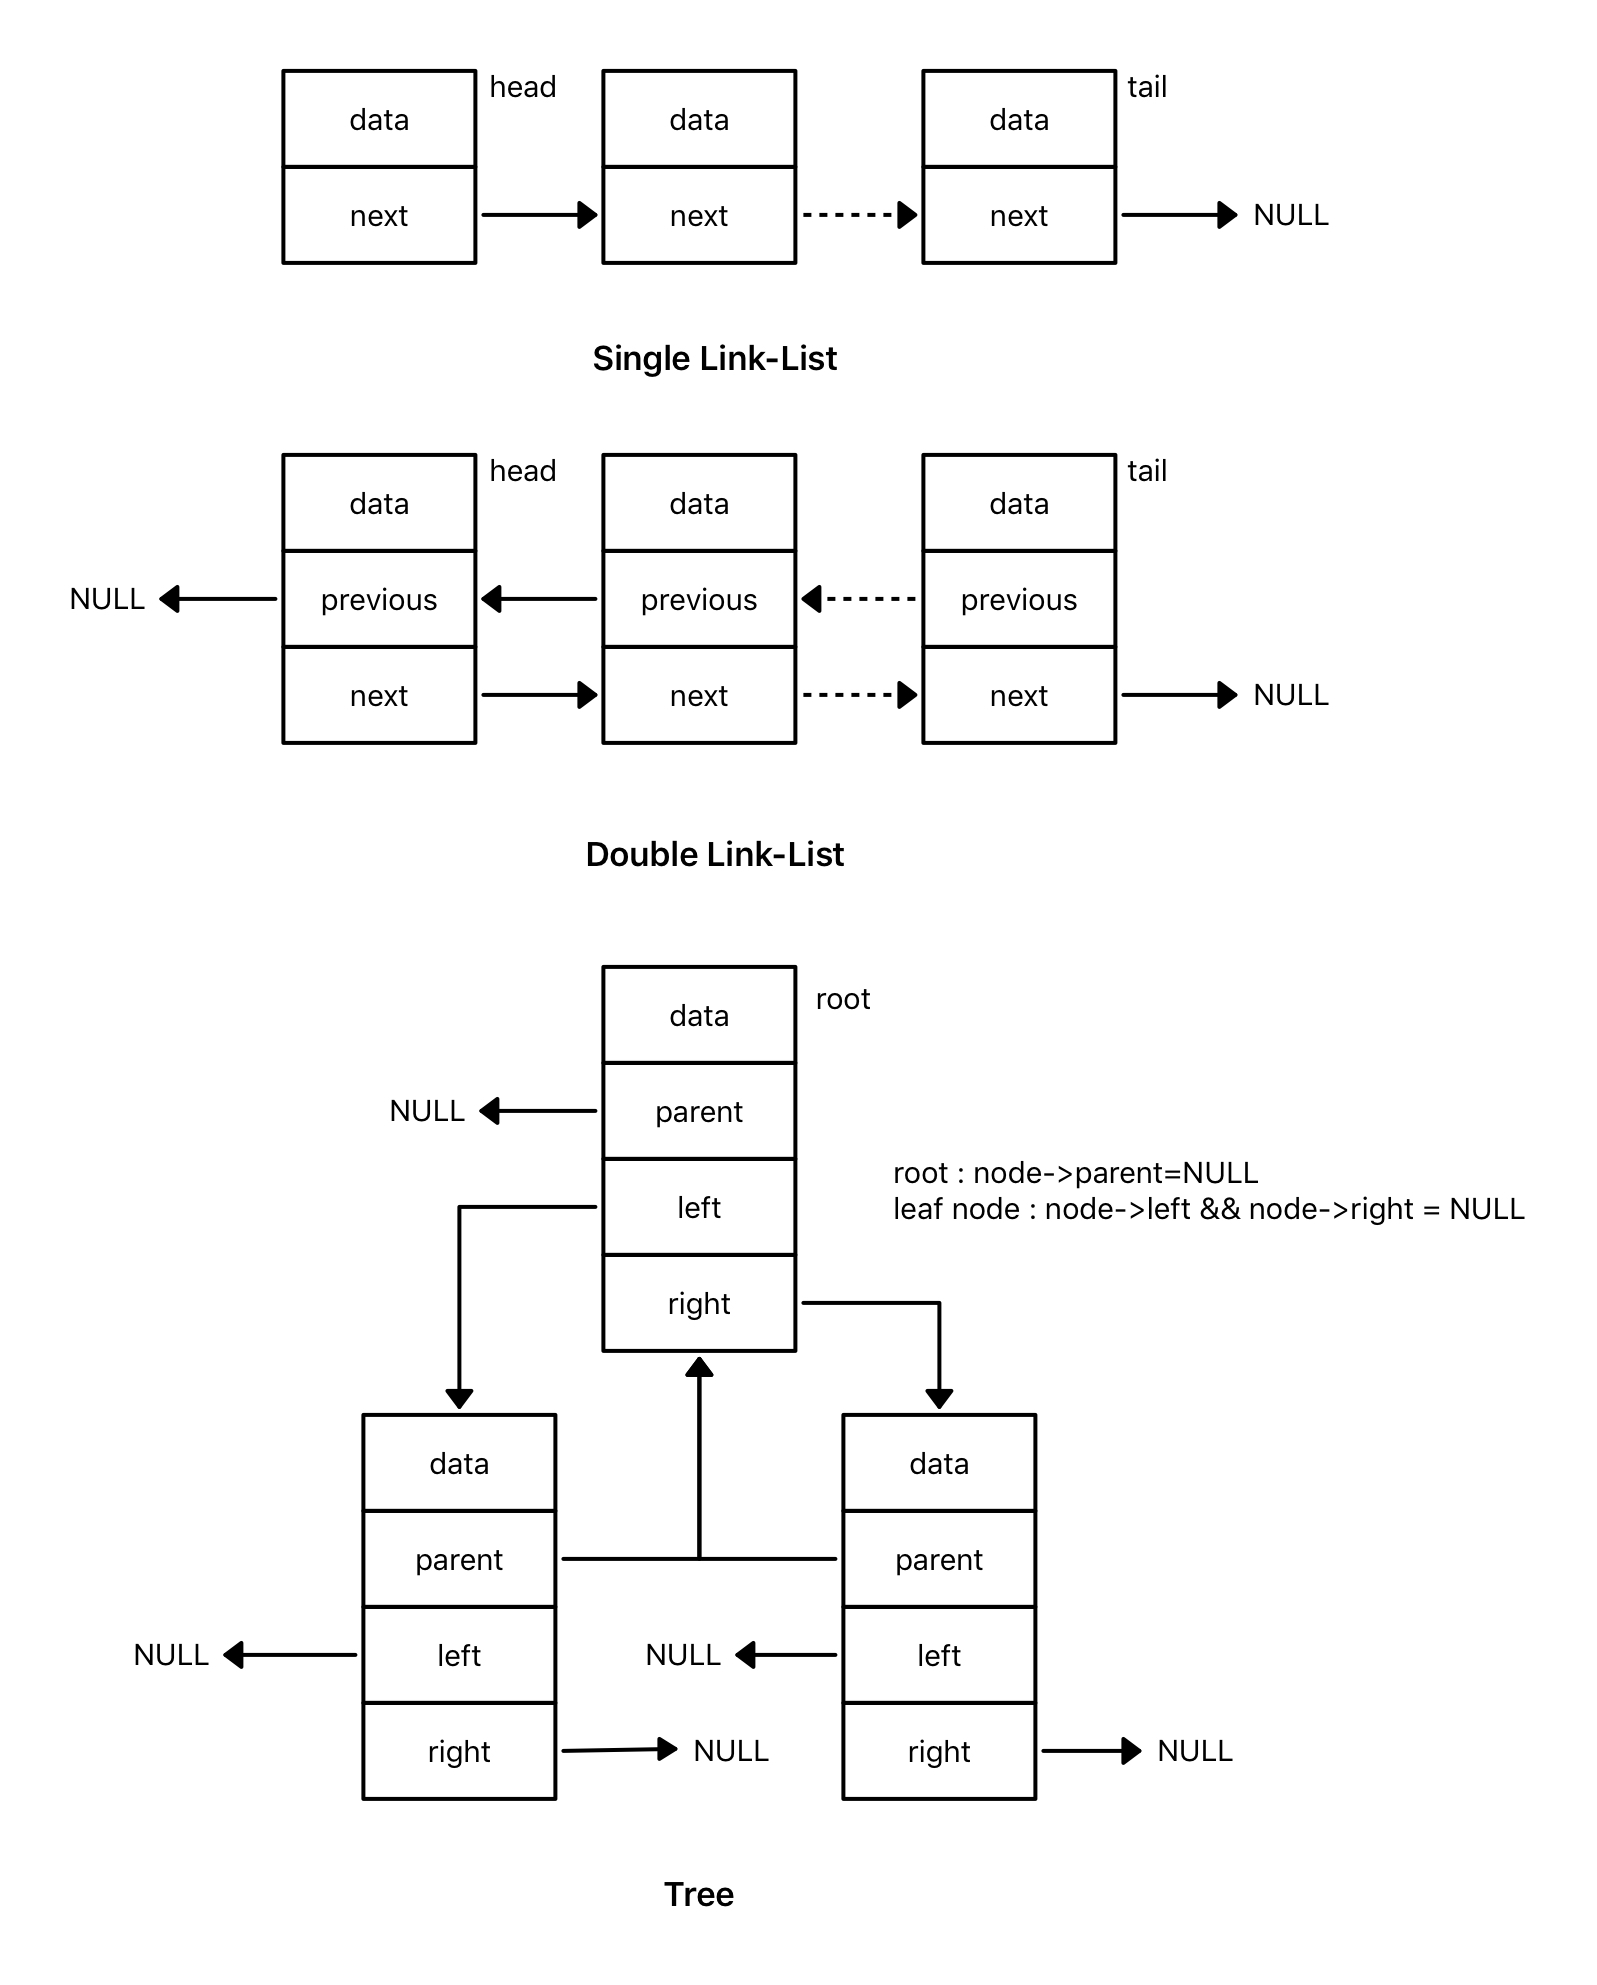
\includegraphics[width=0.8\textwidth]{newlists.jpg}}
\caption{Linked lists: (Top) Single LL (Middle) Double LL (Bottom) Tree}
\label{list}
\end{figure}

Figure \ref{list} show three types of data structure. The first is a single linked list that is unidirectional, next a double linked list that is bidirectional and finally a complete tree which is slightly more complex.

\subsubsection{Single linked lists}

A single linked list is a list structure where there is a single pointer pointing to the address of the next node in the list. The last node is identified as the node which points to NULL. Nodes can be inserted but all scans have to start from the beginning of the list.\\

\begin{lstlisting}[language=C,,showstringspaces=false,caption={File: llist1.c, single linked list},captionpos=b,label=linklist1]
 1 #include <stdio.h>
 2 #include <stdlib.h>
 3 #include <assert.h>
 4 
 5 typedef struct node
 6 {
 7 int data;
 8 struct node *next;
 9 } node_str;
10 
11 #define NEXT(s) s->next
12 #define DATA(s) s->data
13 
14 node_str *create_node(int value)
15 {
16 node_str *ptr;
17 
18 ptr = (node_str*)malloc(sizeof(node_str));
19 
20   if (ptr==NULL)
21   {
22   perror("failed to allocate memory");
23   exit(EXIT_FAILURE);
24   }
25 
26 DATA(ptr) = value;
27 NEXT(ptr) = NULL;
28 return ptr;
29 }
30 
31 void display(node_str *n)
32 {
33 assert(n!=NULL);
34 
35 printf("Single Linked list \n");
36   do
37   {
38   printf("... addr : 0x%8.8x\n",(unsigned int)n);
39   printf("... data : %d\n",DATA(n));
40   printf("... next : 0x%8.8x\n\n",(unsigned int)NEXT(n));
41   n = NEXT(n);
42   }
43   while (n!=NULL);
44 }
45 
46 int main(void)
47 {
48 node_str *root;
49 
50 root=create_node(1);
51 NEXT(root) = create_node(2);
52 NEXT(NEXT(root)) = create_node(3);
53 
54 display(root);
55 
56 free(NEXT(NEXT(root)));
57 free(NEXT(root));
58 free(root);
59 return 0;
60 }

INTERACTIONS

$ cc llist1.c
$ ./a.out
Single Linked list 
... addr : 0xc9c02610
... data : 1
... next : 0xc9c02620

... addr : 0xc9c02620
... data : 2
... next : 0xc9c02630

... addr : 0xc9c02630
... data : 3
... next : 0x00000000
$
\end{lstlisting}

Listing \ref{linklist1} shows the code that creates a single linked list of three nodes. Each node points to the next node in succession. As mentioned previously the last node points to NULL indicating that it is the last node in the list. 

Line:11:12 are useful macros that help with the linked list as it can get confusing when dealing with more complicated structures.

The first root node(1) is created and the data value set to 1. Then the pointer to next node(1) is assigned to the newly created node(2). This is repeated one more time until there is a linked list of three nodes created with each node pointing to the next.  

Finally we can see the output from the program and how the addresses relate to a single linked list. The root node is denoted by the data value 1 and the last node is denoted with data value 3.

\subsubsection{Double linked lists}

A double linked list is exactly as it sounds. In addition to a single link to the next node there is another link to the previous node. This gets around the problem of scanning from the beginning of the list each time a specific node needs to be found or modified. This is useful when there are many nodes and lots of editing occurs on those nodes. 

With single linked lists there is only one unique node which is the last node that points to NULL. By contrast a double linked list has two unique nodes. The first node which has its previous pointer pointing to NULL and the last node.

\begin{lstlisting}[language=C,caption={File: llist2.c, double linked list},showstringspaces=false,captionpos=b,label=linklist2]

 1 #include <stdio.h>
 2 #include <stdlib.h>
 3 #include <assert.h>
 4 
 5 typedef struct node
 6 {
 7 int data;
 8 struct node *previous;
 9 struct node *next;
10 } node_str;
11 
12 #define NEXT(s) s->next
13 #define LAST(s) s->previous
14 #define DATA(s) s->data
15 
16 node_str *create_node(int value)
17 {
18 node_str *ptr;
19 
20 ptr = (node_str*)malloc(sizeof(node_str));
21 
22   if (ptr==NULL)
23   {
24   perror("failed to allocate memory");
25   exit(EXIT_FAILURE);
26   }
27 
28 DATA(ptr) = value;
29 NEXT(ptr) = NULL;
30 LAST(ptr) = NULL;
31 return ptr;
32 }
33 
34 void display(node_str *n)
35 {
36 assert(n!=NULL);
37 
38 printf("Double Linked List \n");
39   do
40   {
41   printf("... addr : 0x%8.8x\n",(unsigned int)n);
42   printf("... data : %d\n",DATA(n));
43   printf("... prev : 0x%8.8x\n",(unsigned int)LAST(n));
44   printf("... next : 0x%8.8x\n\n",(unsigned int)NEXT(n));
45   n = NEXT(n);
46   }
47   while (n!=NULL);
48 }
49 
50 int main(void)
51 {
52 node_str *root;
53 
54 root=create_node(1);
55 NEXT(root) = create_node(2);
56 LAST(NEXT(root)) = root;
57 NEXT(NEXT(root)) = create_node(3);
58 LAST(NEXT(NEXT(root))) = NEXT(root);
59 display(root);
60 
61 free(NEXT(NEXT(root)));
62 free(NEXT(root));
63 free(root);
64 
65 return 0;
66 }

INTERACTIONS

$ cc llist2.c
$ ./a.out
Double Linked List 
... addr : 0x41c02610
... data : 1
... prev : 0x00000000
... next : 0x41c02630

... addr : 0x41c02630
... data : 2
... prev : 0x41c02610
... next : 0x41c02650

... addr : 0x41c02650
... data : 3
... prev : 0x41c02630
... next : 0x00000000
$

\end{lstlisting}

Listing \ref{linklist2} shows the code for a double linked list. It is similar to a single linked list but it includes an extra pointer to the previous node, as defined on line:8. Every time a node is added to the list both the previous link and the previous node's next link are updated. 

Double linked lists allow for a cursor-like concept, we can scan forwards as well as backwards within the list. To insert a new list into an existing list requires only 4 links to be updated. The links connected to the nodes around the insertion point in the original list. As well as the links in the head and tail of the new list require updating. This technique allows large insertions without major modifications to the original structure.  

\subsubsection{Tree}

A tree is a hierarchical structure where each node can have multiple child nodes, normally referred to as the left and right children in the case of a binary tree. A tree can be searched in multiple ways, for example depth-first or breadth-first. There are three traversal order available when search trees i.e. infix, postfix and prefix. This is best illustrated with an example. 

If we use a simple tree with 3 nodes, a parent node and two child nodes i.e. left and right. The parent is the + operator and the left child is x and the right child is y. A infix traversal order would be x + y, postfix traversal order is x y + and finally the prefix traversal is + x y. The traversal order is the order the nodes are visited. This is particularly useful when evaluating and dealing with expressions.

\begin{lstlisting}[language=C,showstringspaces=false,caption={File: llist3.c, binary tree structure},captionpos=b,label=linklist3]

 1 #include <stdio.h>
 2 #include <stdlib.h>
 3 #include <assert.h>
 4 
 5 typedef struct node
 6 {
 7 int data;
 8 struct node *parent;
 9 struct node *left;
10 struct node *right;
11 } node_str;
12 
13 #define LEFT(s)   s->left
14 #define RIGHT(s)  s->right
15 #define PARENT(s) s->parent
16 #define DATA(s)   s->data
17 #define LEFTSIDE  1
18 #define RIGHTSIDE 2
19 
20 node_str *create_node(int value)
21 {
22 node_str *ptr;
23 
24 ptr = (node_str*) malloc(sizeof(node_str));
25 
26   if (ptr==NULL)
27   {
28   perror ("failed to allocate memory");
29   exit (EXIT_FAILURE);
30   }
31 
32 DATA(ptr)   = value;
33 LEFT(ptr)   = NULL;
34 RIGHT(ptr)   = NULL;
35 PARENT(ptr) = NULL;
36 return ptr;
37 }
38 
39 void display (node_str *n)
40 {
41   if (n==NULL) return;
42 
43   printf ("... addr   : 0x%8.8x\n",(unsigned int)n);
44   printf ("... data   : %d\n",DATA(n));
45   printf ("... parent : 0x%8.8x\n",(unsigned int)PARENT(n));
46   printf ("... left   : 0x%8.8x\n",(unsigned int)LEFT(n));
47   printf ("... right  : 0x%8.8x\n\n",(unsigned int)RIGHT(n));
48   
49   display (LEFT(n));
50   display (RIGHT(n));
51 }
52 
53 void free_tree(node_str *n)
54 {
55   if (n==NULL) return;
56 
57 free_tree(LEFT(n));
58 free_tree(RIGHT(n));
59 
60 printf ("... free(ing) 0x%8.8x\n",(unsigned int)n);
61 free(n);
62 }
63 
64 node_str *attach(node_str *r,node_str *a, int mode)
65 {
66 assert ((mode==LEFTSIDE) ||  (mode==RIGHTSIDE));
67 assert (r!=NULL);
68 assert (a!=NULL);
69 
70   switch(mode)
71   {
72   case LEFTSIDE:
73   LEFT(r) = a;
74   break;
75 
76   case RIGHTSIDE:
77   RIGHT(r) = a;
78   break;
79   }
80 
81 PARENT(a) = r;
82 return a;
83 }
84 
85 int main (void)
86 {
87 node_str *root;
88 node_str *tmp;
89 
90 root=create_node (1);
91 tmp = attach (root,create_node(2),LEFTSIDE);
92 tmp = attach (root,create_node(3),RIGHTSIDE);
93 attach (tmp,create_node(4),LEFTSIDE);
94 
95 printf ("Binary Tree Linked list \n");
96 display (root);
97 free_tree(root);
98 
99 return 0;
100 }

INTERACTIONS

$ cc llist3.c
$ ./a.out
Binary Tree Linked list 
... addr   : 0xb5402610
... data   : 1
... parent : 0x00000000
... left   : 0xb5402630
... right  : 0xb5402650

... addr   : 0xb5402630
... data   : 2
... parent : 0xb5402610
... left   : 0x00000000
... right  : 0x00000000

... addr   : 0xb5402650
... data   : 3
... parent : 0xb5402610
... left   : 0xb5402670
... right  : 0x00000000

... addr   : 0xb5402670
... data   : 4
... parent : 0xb5402650
... left   : 0x00000000
... right  : 0x00000000

... free(ing) 0xb5402630
... free(ing) 0xb5402670
... free(ing) 0xb5402650
... free(ing) 0xb5402610
$
\end{lstlisting}

Listing \ref{linklist3} implements a tree with two children. Each node contains three pointers. A left and right link to each child and a parent link pointing to the parent node. 

A leaf node is identified as having no children, i.e. both left and right pointers are NULL (see nodes(2) and (4)). The root node(1) is the node where the parent link points to NULL. 

This program uses recursion for both \textit{display(...)} and \textit{free\_tree(...)} functions. Recursion is a Computer Science technique where a function calls itself. The \textit{display(...)} function uses a prefix top-down recursive algorithm whereas \textit{free\_tree(...)} function uses a postfix bottom-up recursive algorithm.

For deeply embedded or safety-critical systems, recursion is discouraged because recursion can require an unknown amount of stack space, also there is the possibility that the result becomes divergent (doesn't come to an end).
